\section{Infrastructure as Code [Mohammed Mehedi Hasan]}\label{sec:infrastructure_as_code}

Azure Resource Manager (ARM) is the native platform for infrastructure as code (IaC) in the Azure virtual cloud. It is a service that allows users to deploy and manage resources using infrastructure as a code paradigm. To deploy and manage resources using ARM, a user needs to create two ARM objects, they are ARM templates and template parameters. The ARM template is a file that defines what resources and how those resources should be deployed to groups, subscriptions, or tenants, and in the template parameters file, a user specifies which values they want to input when deploying the resources. Both of these files are defined in JavaScript Object Notation (JSON) and have a declarative syntax defined by Microsoft. Following the paradigm defined by azure, for this CD pipeline solution, an ARM template file was created that first creates a resource group in the Azure portal which will contain any further resources then it provisions an AKS cluster. The parameters file defines some inputs like Cluster name, DNS prefix, etc. Primarily the ARM template creates an AKS cluster with just one node machine but the template also enables the auto-scaling feature of AKS and sets the maximum cluster node count to three. ARM template task in the CD pipeline performs an incremental build, which means that the AKS cluster is not redeployed every time the CD pipeline executes, it only updates the cluster if necessary after the first build. It saves a huge amount of computing resources and time since provisioning an AKS cluster takes a significant amount of time. 

\subsection{Load-balancing Architecture}
Since this CI-CD implementation of the spring boot application deploys the app in a Kubernetes environment, it takes advantage of Kubernetes advanced load balancing capabilities. ARM provisions an AKS cluster that is capable of scaling up to three-node machines when the traffic is high ~\ref{fig:arm_laodbalancing} , this architecture is further extended using Kubernetes deployment objects. In the AKS  cluster, the spring boot app deployment object creates and maintains at least three running replicas of the application pods. In case of any pod failure, Kubernetes API will remove and regenerate a new pod to replace it, so the application always serves requests using at least three pods. However, for the PostgreSQL deployment object in AKS, the default and maximum replica count is set to one thus there's always just one PostgreSQL deployment that opens a connection to all three application pods.

Then both the application deployment and PostgreSQL deployment are exposed as a ClusterIP service object. ClusterIP service ensures that the application and database are not reachable from outside of the cluster but the pods inside the cluster in the same namespace can communicate with each other. The application service is then exposed using a reverse proxy service called Nginx. Nginx implements Kubernetes ingress resource with a round-robin load balancing architecture. Ingress Nginx creates an externally accessible public IP address in the cluster and exposes the application service in HTTP and HTTPS ports. Finally, an FQDN is configured from the Azure portal from which performs DNS name resolution on the external IP produced by ingress. After that, the spring boot application is reachable from that FQDN.

The ingress Nginx balances the incoming traffic to the available application pods dynamically. If the incoming traffic increases to a level where the AKS cluster has created many replicas of the application pod and thus exhausted the resources of one available node machine of the cluster then AKS will automatically scale up the node pool and deploy another node machine with any human assistance. Then additional pods of the same application deployment will be dynamically created in the new node to server further requests. When the traffic level decreases, AKS will automatically scale down the node pool to one machine and save computing resources.

\begin{figure}
    \centering
    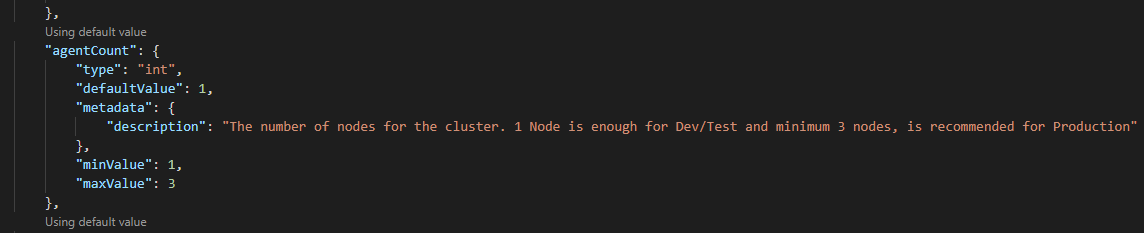
\includegraphics[width=14cm]{images/Rahat/ARM-LB.PNG}
    \caption{ARM Load-Balancing}
    \label{fig:arm_laodbalancing}
\end{figure}